
\documentclass[12pt,reqno]{amsart}

\usepackage{graphicx}

\usepackage{amssymb}
\usepackage{amsthm}
\theoremstyle{plain}

\newtheorem*{theorem*}{Theorem}
%% this allows for theorems which are not automatically numbered

\newtheorem{definition}{Definition}
\newtheorem{theorem}{Theorem}
\newtheorem{lemma}{Lemma}
\newtheorem{example}{Example}
\newtheorem*{normal}{Normal Play}
\newtheorem*{variations}{Variations}
\newtheorem*{solution}{Solution}
\newtheorem*{introduction}{Introduction}
\newtheorem{conjecture}{Conjecture}
\usepackage{lineno}
\usepackage{etoolbox}
\makeatletter
\patchcmd{\@maketitle}
  {\ifx\@empty\@dedicatory}
  {\ifx\@empty\@date \else {\vskip3ex \centering\footnotesize\@date\par\vskip1ex}\fi
   \ifx\@empty\@dedicatory}
  {}{}
\patchcmd{\@adminfootnotes}
  {\ifx\@empty\@date\else \@footnotetext{\@setdate}\fi}
  {}{}{}
\makeatother

\title{Development of Two-Player Tower of Hanoi Variation with Cyclic Behaviour}
\author{Jansher Azmat}
\date{May 2022}
\begin{document}

\begin{abstract}
Under traditional rules, Tower of Hanoi is a one-player game well-regarded as an introduction to recursive algorithms, proof by induction, and complexity theory. Several variations of the puzzle have since spawned with countless implications to the field of combinatorial game theory. As such, this paper aims to develop a two-player Tower of Hanoi variation that serves as an intuitive and computationally-efficient median to explore the theory of deterministic, perfect-information partisan cyclic games.
\end{abstract}

\maketitle

\section{Classical Tower of Hanoi}
In conventional one-player Tower of Hanoi, the board of play is composed of $3 \ pegs$ and $n \ disks$ of unique sizes stacked on the $starting \ peg$ by increasing order of diameter, with the largest disk forming the $base$. The remaining two pegs are delegated as the $target \ peg$ and $auxiliary \ peg$, respectively. The objective is to relocate the entire stack of $n$ disks from the starting peg to target peg, using the auxiliary peg as an intermediary when necessary, subject to the following restrictions: only the topmost disk of a peg, if existent, can be moved, and no disk can be placed on top of a disk of smaller diameter. A recursive solution to the minimum number of moves required to transfer a tower of $n$ disks was established soon after the game’s inception and remains a relevant result—the algorithm is provided below.
\begin{solution}
Minimum moves to complete classical Tower of Hanoi (Java)
\break
\begin{verbatim}
\\Available at: https://github.com/JansherA/MMResearchPaper

class TowerOfHanoi {
 
  public static void main(String[] args) {
    board(3, 'A', 'B', 'C');
  }
 
  private static void board(int n, char startingPeg, char auxiliaryPeg, 
  char targetPeg){
 
 
    if(n==1){
    
      System.out.println("Move disk 1 from "+startingPeg+" to "+targetPeg);
      return;
    }
 
    board(n-1,startingPeg,targetPeg,auxiliaryPeg);
 
    System.out.println("Move disk "+n+" from "+startingPeg+" to "+targetPeg);
 
    board(n-1,auxiliaryPeg,startingPeg,targetPeg);
    
  }
}

\end{verbatim}
\end{solution}
\section{Variations}
\begin{variations} \normalfont
As aforementioned, two-player variations of Tower of Hanoi have been widely studied for their applications to combinatorial game theory; the most recognized of which retain the game’s objective and two fundamental rules while further generalizing the structure of play as follows:

\begin{definition}
Two players exchange turns individually transferring $n$ disks from the initial stack across $k$ pegs and onto the target peg in increasing order, such that the winning player completes the transfer by placing the smallest disk atop $n-1$ disks on the target peg. 
\end{definition}
Indeed, this ending condition produces a deterministic perfect information game whereby the first player to move always wins. Accordingly, alternate winning conditions have been adopted in order to achieve second-player wins, although such strategies have proven largely unsuccessful. Importantly, this is due to the game’s inherent cyclical nature: the first player to move controls the state of the game and dictates the other player’s moves, whom can at best accept a tie by forcing an infinite loop of moves in certain existing variations. Thus, a new version of the game is established with potential for interesting second-player results.

\end{variations}
\section{Red-Blue Tower of Hanoi}
In Red-Blue Tower of Hanoi, the familiar setup is reduced in generality, and color-coded disks now correspond to the two players as detailed below:

\begin{definition}
A game of Red-Blue Tower of Hanoi is set up with four pegs and a set of three discs placed on each exterior peg. The first peg contains three blue discs of unique diameters positioned in increasing order of size with the largest disc forming the base. The fourth peg consists of three red discs oriented identically. The second and third pegs are left empty. Two players, Red and Blue, control their respective stack of discs and aim to transfer it to any of the remaining three pegs according to the standard Tower of Hanoi rules. A player can place a disc on an opposite colored disc so long as the disc moved does not equal or exceed the size of the disc it is placed on top of. The first player to successfully transfer their tower to a peg other than its location of origin is deemed the winner, and an infinite loop of moves is considered a tie. Starting moves are limited to placing the smallest disc on either the second or third peg. Sample games and end positions are provided below.
\end{definition}
\begin{example}
Red-Blue Tower of Hanoi set up:
\begin{figure}[htp]
    \centering
    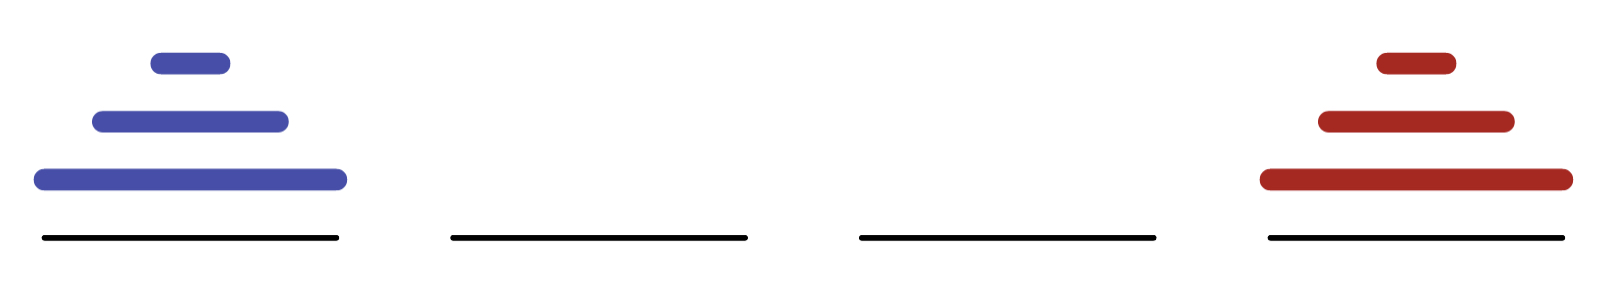
\includegraphics[width=13cm]{modern1.jpg}
    \caption{Red-Blue Tower of Hanoi Starting Position}
    \label{fig:Starting position}
\end{figure}
\end{example}
\begin{example}
Red player winning position:
\begin{figure}[htp]
    \centering
    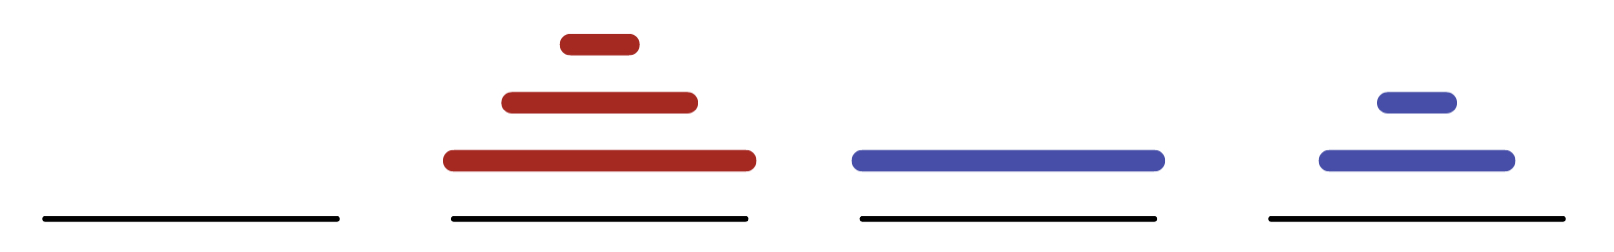
\includegraphics[width=13cm]{modern2.jpg}
    \caption{Red-Blue Tower of Hanoi Red Win}
    \label{fig:Red Win} 
\end{figure}
\end{example}
\break
\begin{example} 


Blue player win:
\begin{figure}[htp]
    \centering
    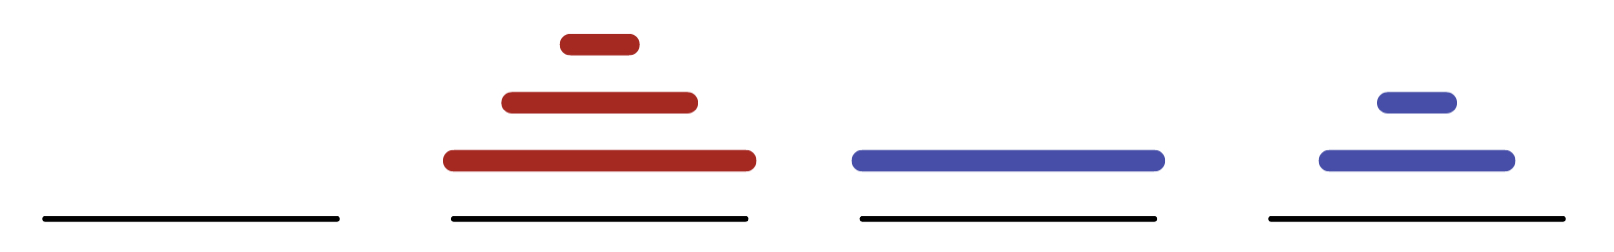
\includegraphics[width=13cm]{modern2.jpg}
    \caption{Red-Blue Tower of Hanoi Blue Win}
    \label{fig:Blue Win}
\end{figure}
\end{example} 
Conjectures for Red-Blue Tower of Hanoi are proposed below. 
\begin{conjecture}
Unlike traditional variations of Tower of Hanoi, the second player in Red-Blue can always force a tie after any starting move from the opponent. To achieve this, suppose the second player in a particular new game is Blue. Following the first move from Red, Blue must react by moving to the remaining open peg. Blue must always place a disc on an empty peg when the option is available, unless a winning end move is present; such a move to occupy an empty peg is called an "Occupy." Otherwise, Blue must aim place the smallest blue disc available on top of any peg where the top disc on said peg is Red; such a move is called a "Block."
\end{conjecture}
By Occupying any empty pegs, Blue prevents Red from starting a new winning stack and thereby increases their control over the game. Red must begin their path to a winning end condition by placing the largest red disc onto an empty beg. Thus, Blue prevents such an opportunity through Occupying by maintaining control over empty pegs. In a situation where Red achieves a position with their largest disc at the bottom of a peg (other than the starting peg), Blue can prevent Red from further developing a red stack by Blocking any such positions. Through Blocking and Occupying, Blue can enter an infinite cycle of denying Red any progression towards a winning end position, thereby deeming the game a tie. As proposed, this conjecture would serve as an improvement over the previous notion that the first player can always win a variation of Tower of Hanoi. 

\begin{conjecture}
Because of the cyclic nature of Red-Blue Tower of Hanoi, whereby the second player can always force an infinite loop of moves, this variation is a suitable candidate for improving disjunctive sum theory for cyclic games. 
\end{conjecture}
Calculating the disjunctive sum of distinct positions of Red-Blue Tower of Hanoi would be computationally-efficient given the game's simplistic nature and easy set up, as opposed to popular existing loopy games. Furthermore, such a brute force analysis could offer nontrivial insights that could possibly extend the Sprague-Grundy Theorem for cyclic impartial games.
\section{References}
\newcounter{boxlblcounter}  
\newcommand{\makeboxlabel}[1]{\fbox{#1.}\hfill}
\newenvironment{boxlabel}
  {\begin{list}
    {\arabic{boxlblcounter}}
    {\usecounter{boxlblcounter}
     \setlength{\labelwidth}{3em}
     \setlength{\labelsep}{0em}
     \setlength{\itemsep}{2pt}
     \setlength{\leftmargin}{1.5cm}
     \setlength{\rightmargin}{2cm}
     \setlength{\itemindent}{0em} 
     \let\makelabel=\makeboxlabel
    }
  }
{\end{list}}



\begin{boxlabel}

\item Andreas M. Hinz. 1992. Shortest paths between regular states of the tower of Hanoi. Inf. Sci. 63, 1–2 (Sept. 1, 1992), 173–181.
\item Chappelon, Jonathan, Urban Larsson, and Akihiro Matsuura. "Two-player tower of hanoi." International Journal of Game Theory 47.2 (2018): 463-486.
\item Fraenkel, Aviezri S., and Yaacov Yesha. "The generalized Sprague-Grundy function and its invariance under certain mappings." Journal of Combinatorial Theory, Series A 43.2 (1986): 165-177.
\item Hayes, P. J. "Discussion and correspondence: A note on the Towers of Hanoi problem." The Computer Journal 20.3 (1977): 282-285.
\end{boxlabel}

\end{document}

